% THIS IS SIGPROC-SP.TEX - VERSION 3.1
% WORKS WITH V3.2SP OF ACM_PROC_ARTICLE-SP.CLS
% APRIL 2009
%
% It is an example file showing how to use the 'acm_proc_article-sp.cls' V3.2SP
% LaTeX2e document class file for Conference Proceedings submissions.
% ----------------------------------------------------------------------------------------------------------------
% This .tex file (and associated .cls V3.2SP) *DOES NOT* produce:
%       1) The Permission Statement
%       2) The Conference (location) Info information
%       3) The Copyright Line with ACM data
%       4) Page numbering
% ---------------------------------------------------------------------------------------------------------------
% It is an example which *does* use the .bib file (from which the .bbl file
% is produced).
% REMEMBER HOWEVER: After having produced the .bbl file,
% and prior to final submission,
% you need to 'insert'  your .bbl file into your source .tex file so as to provide
% ONE 'self-contained' source file.
%
% Questions regarding SIGS should be sent to
% Adrienne Griscti ---> griscti@acm.org
%
% Questions/suggestions regarding the guidelines, .tex and .cls files, etc. to
% Gerald Murray ---> murray@hq.acm.org
%
% For tracking purposes - this is V3.1SP - APRIL 2009

\documentclass{acm_proc_article-sp}

\usepackage{multirow}
\usepackage{subfigure}
\usepackage{graphicx}
\usepackage{graphics}
\usepackage{rotating}
\usepackage{verbatim}
\usepackage{float}
\usepackage{url}

\usepackage{listings}
\usepackage{color}
\definecolor{javared}{rgb}{0.6,0,0} % for strings
\definecolor{javagreen}{rgb}{0.25,0.5,0.35} % comments
\definecolor{javapurple}{rgb}{0.5,0,0.35} % keywords
\definecolor{javadocblue}{rgb}{0.25,0.35,0.75} % javadoc
 
\lstset{language=Java,
basicstyle=\ttfamily,
keywordstyle=\color{javapurple}\bfseries,
stringstyle=\color{javared},
commentstyle=\color{javagreen},
morecomment=[s][\color{javadocblue}]{/**}{*/},
%numbers=left,
numberstyle=\tiny\color{black},
stepnumber=2,
numbersep=10pt,
tabsize=4,
showspaces=false,
showstringspaces=false}



\restylefloat{table}
\hyphenation{op-tical net-works semi-conduc-tor}
\begin{document}

\title{Automated Discovery of Failure Domain}

\numberofauthors{2} %  in this sample file, there are a *total*
% of EIGHT authors. SIX appear on the 'first-page' (for formatting
% reasons) and the remaining two appear in the \additionalauthors section.
%
\author{
% You can go ahead and credit any number of authors here,
% e.g. one 'row of three' or two rows (consisting of one row of three
% and a second row of one, two or three).
%
% The command \alignauthor (no curly braces needed) should
% precede each author name, affiliation/snail-mail address and
% e-mail address. Additionally, tag each line of
% affiliation/address with \affaddr, and tag the
% e-mail address with \email.
%
% 1st. author
\alignauthor
Mian Asbat Ahmad\\
       \affaddr{Department of Computer Science}\\
       \affaddr{University of York}\\
       \affaddr{York, United Kingdom}\\
       \email{mian.ahmad@york.ac.uk}
% 2nd. author
\alignauthor
Manuel Oriol \\
       \affaddr{Department of Computer Science}\\
       \affaddr{The University of York}\\
       \affaddr{York, United Kingdom}\\
       \email{manuel.oriol@york.ac.uk}
}


\maketitle
\begin{abstract}
Many research studies in the random testing literature refer to 
point, block and strip fault domains across the input domain of a system.
A number of new strategies have also been devised on this principle claiming better results.
However, no study was conducted to graphically show their existence
and the frequency of each faulty domain in real production application. 

In this research we study fault domains and check to which type of domains they belong. 
Our experimental results show that in 60\%  cases faults form point domain, 
while block and strip domain form 20\% each. We also checked what relation exists 
between fault domains traced back to only one fault: are they contiguous, separate, or marginally adherent. 

This study allows for a better understanding of fault domains and assumptions made on the 
strategies for testing code. We applied our results by correlating our study with three random strategies: random, random+ and DSSR. 

\end{abstract}


\category{D.2.5}{Software Engineering}{Testing and Debugging}[Testing Tools, Failure Domains, Random testing, Automated Testing]

\section{Introduction}\label{sec:intro}

Testing is fundamental requirement to assess the quality of any software. Manual testing is labour-intensive and error-prone; therefore emphasis is to use automated testing that significantly reduces the cost of software development process and its maintenance \cite{Beizer1995}. Most modern black-box testing techniques execute the System Under Test (SUT) with specific input and compare the obtained results against the test oracle. A report is generated at the end of each test session containing any discovered faults and the input values which triggers the faults. Debuggers fix the discovered faults in the SUT with the help of these reports. The revised version of the system is given back to the testers to find more faults and this process continues till the desired level of quality, set in test plan, is achieved.

The fact that exhaustive testing for any non-trivial program is impossible, compels the testers to come up with some strategy of input selection from the whole input domain. Pure random is one of the possible strategies that are widely used in automated tools. It is intuitively simple, easy to implement, minimum or no overhead in input selection and lack of bias \cite{Ciupa2008, Forrester2000, Hamlet1994, Linger1993}. While pure random testing has many benefits there are also some limitations that include low code coverage \cite{Offutt1996} and discovery of lower number of faults \cite{Chen1994}. To overcome these limitations many researchers successfully refined pure random testing while keeping its benefits intact. Most significant refinement of random testing is Adaptive Random Testing (ART) \cite{Chen2008}. The experiments performed using ART showed up to 50\% better results as compared to the traditional/pure random testing which has no criteria for input selection.  Similarly Restricted Random Testing (RRT), Mirror Adaptive Random Testing (MART), Adaptive Random Testing for Object Oriented Programs (ARTOO), Directed Adaptive Random Testing (DART), Lattice-based Adaptive Random Testing (LART) and Feedback-directed Random Testing (FRT) \cite{Chan2006, Chen2004, Ciupa2008,  Godefroid2005, Mayer2005, Pacheco2007} are some of the variations of random testing aiming to increase the overall performance of pure random testing.

\begin{figure}[h]
\centering
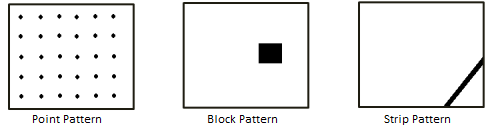
\includegraphics[width=8cm,height=2.5cm]{ART_Patterns.png}
\caption{Failure domains across input domain \cite{Chan1996}}
\label{fig:patterns}
\end{figure}


All the above mention variations in random testing are based on the observation that failure causing inputs across the whole input form certain kinds of domains \cite{Chan1996}.  They divided them into point, block and strip fault domain. In Figure \ref{fig:patterns} the square box represents the whole input domain while the black point, block and strip inside the box represent the faulty values across the input domain. They further suggested that the effectiveness of testing could be improved by taking into account the possible characteristics of failure causing inputs.



% It is important to note that these techniques only identify a single instance of failure and do not  focus on the failure domain. 

%2.	It is also noticed that further analysis of fault lead to new faults which the testing process may not have identified.
%3. 	Experiments can be performed to analyse the frequency of existence of point, block and strip domain across the input domain. 

%Random testing is a black-box testing technique in which parts (methods/modules) of SUT are selected randomly and then executed against randomly generated test data from the whole input domain. Results obtained from the execution are either compared to the specifications of the SUT or language exceptions which served as a test oracle. Any test output that fail to meet the oracle either because of failing to comply the specification or trigger the exceptions are considered as potential faults. In this paper we present a new tool, called Automated Discovery of Failure Domain (ADFD), based on a random testing tool called York Extensible Testing Infrastructure (YETI), for not only finding fault but also its domain. ADFD utilise YETI to discover the fault in the given SUT and then generate a dynamic code for finding its domain. The found domain -- point, block or strip are presented on the graph at the end of each test session


%ADFD has been designed to decrease the time of system testing. Knowing the domain of the fault the debuggers This research can decrease the overall testing time by reducing the number of code exchanges between testers and debugger. It is achieved by tracking the failure domain and not only a single instance failure. Tracking failure domain provide more information about the behaviour of the fault.

%that also served as regression testing. None of the testing techniques evaluate the nature of the fault and the pattern in which the fault reside. 


%The aim of this research study is to find not only find the values for which the system fails but also the domains of failure causing inputs which will help in automated generation of fault targeted test cases for any black-box testing technique.\\


%Over the past few years there is a tremendous growth in development of hardware whose main focus is to increase the computer processing power. The computers that served as a mini and mainframe computers few years ago are turned into personal computer in todays modern age. To utilise this processing power various software development companies started to develop more sophisticated and processing hungry softwares. These softwares provide simple and easy to use Graphical User Interface (GUI) but on the back end they are equally complex and consist of thousands of instructions. This increase in size of the software also increases the difficulty of preserving high quality, reliability, portability, maintainability and efficiency of the software. These problems are mainly cater by software testing. The increase of complexity and size of softwares also forced the researchers to find new ways of software testing that are more efficient, reliable and speedy to cope with the ever increasing hardware and software industry.\\

%Mirror Adaptive Random Testing (MART)  \cite{Chen2003}, Feedback-directed Random Testing (FDRT) \cite{Pacheco2007}, Restricted Random Testing (RRT) \cite{Chan2002} and Quasi Random Testing  (QRT) \cite{Chen2005} are the strategies based on the same principle that found better results compared to ordinary random testing.

It is interesting that where many random strategies are based on the principal of contiguous fault domains inside the input domain no specific strategy is developed to evaluate these fault domains. This paper describes a new test strategy called Automated Discovery of Failure Domain (ADFD). The ADFD strategy not only finds the fault but also finds its domain. The idea of identification of fault domain is attractive as it provides an insight of the fault domains in the SUT. Additionally, the paper makes the following contributions:

\begin{itemize}
\item \textbf{Implementation:} It presents the implementation of the new ADFD strategy in York Extensible Testing Infrastructure (YETI) tool.
\item \textbf{Evaluation:} Several classes are tested with ADFD strategy to evaluate its behaviour.
\item \textbf{Decrease in Test Duration:} Identification of the fault domain instead of a single instance of fault decreases testing times by reducing the back and forth of the project between testers and debuggers
\item \textbf{Increase in Test Efficiency:} ADFD strategy helps debugger team as the debuggers will keep in view all the fault occurrences while \end{itemize}



% Additionally, ADFD test strategy can also be used to identify frequency of point, block and strip fault domain across the production softwares.



%The main objective behind ADFD is to get an automated frame work that find the existence of fault and fault domain across the input domain, decrease debugging time and to discover any more faults missed by the testing system. Significant research has been done to utilise the failure domains but their existence, nature and boundaries need further attention. Having fault domain information prior to testing enables the tester to guide testing according to the failure domain of the SUT, for example pure random testing is more effective for point domain than block and strip domains where as ART, MART, FDRT, RRT and QRT are more effective for block and strip fault domains than point fault domain.

%In our previous research we extended the same idea of the existence of different domains of failure across the whole input domain proposed by Chen et al, \cite{Chen2008} and accepted by various other researchers to develop a new strategy called Dirt Spot Sweeping Strategy [X]. However the experimental results showed not very considerable improvement then what we predicted. We performed 500 experiments in which we carried out 10000 tests but the results showed only 5\% improvement contrary to our prediction of 30\%. All the experiments were performed from a pool of open-source projects bundled in a repository called Qualitas Corpus \cite{Tempero2010}. Corpus contains more than 100 open-source java projects and maintained only for the purpose of unbiased research experiments. Therefore one of the conclusions derived from our experiments was that the patterns of failure may not exist in most of the software’s due to which our strategy which focus on these patterns didn’t produce much efficiency.\\
%It was therefore very interesting for us to do further research to find about the existence and nature of these failure patterns. Our main focus in this research paper is to discover whether there exist failure patterns across the input domain or not and if they exist then how frequent and what pattern they follow.\\

The rest of this paper is organized as follows: \\ Section~\ref{sec:adfd} describes the ADFD strategy. Section~\ref{sec:implementation} presents implementation of the ADFD strategy. Section~\ref{sec:experimentalResults} explains the experimental results. Section~\ref{sec:discussion} discusses the results. Section~\ref{sec:relatedWork} presents related work and Section~\ref{sec:conclusion}, concludes the study.

%In Section II, we describe the automated discovery of failure domain test strategy and explain its structure and function with the help of a flowchart and motivating example. Section III presents its implementation in automated random testing tool called York Extensible Testing Infrastructure (YETI). Section IV and V report the experiments performed using the proposed technique and evaluate \& discuss the obtained results. Section VI and VII discuss any threats to validity and related discussion. Finally we conclude in Section VIII. 

%The rest of this paper is organized as follows. The sections, II to X, describe automated strategy, Implementation, Experimental setup and analysis, Evaluation, Experimental results, discussion, conclusion and future work respectively.\\

%X\section{Problems and Solutions}\label{sec:probl_and_sol}
%This paper address five. main problems in random testing. These are (1) Finding the whole domain of fault instead of only failing values, (2) Representation of fault values, (3) automation of the evaluation process, (4) Identification of fault domain for multi arguments methods and its representation, (5) Generation and classification of test values for Strings and complex (non scaler) arguments. This section elaborate each of the above mention problem and describe our proposed solution (if any) to them.

%\subsection{Finding the whole domain of fault instead of only failing values}
%Most of the testing tools take into account only the fault finding values with out giving due consideration to the domain in which the values exist. \subsection{Representation of fault values and fault domains}
%points: instead of dumping logs and more complex reports we describe the fault domains with the help of charts. 
%\subsection{Automation of the testing process}
%We developed an automated system to test the system, generate the fault domain finding files, compile and execute them to find the fault domains if any. points: automation is achieved by combining the test tool and evaluation system e.g. yeti and ADFD.   
%\subsection{Identification and representation of multi arguments data}
%I think it is beyond the scope of this study to identify and represent more then 3 arguments method because at the moment we can show only three diminutional charts.
%\subsection{Generation and classification of test values for string and complex (non scaler) arguments}
%It is difficult to find the domain for strings and complex (non scaler) data therefore they can be exempted from this study.


\section{Automated Discovery of Failure Domain}\label{sec:adfd}

Automated Discovery of Failure Domain (ADFD) is a new test strategy where testing of SUT starts using Random+ (R+) strategy to find not only the fault but its complete domain across the whole input domain. The output produced at the end of test session is an (x,y) chart showing the passing value or range of values in green line and failing value or range of values in red line. The work flow of ADFD strategy is given in Figure \ref{fig:ADFD}.

\begin{figure}[ht]
\centering
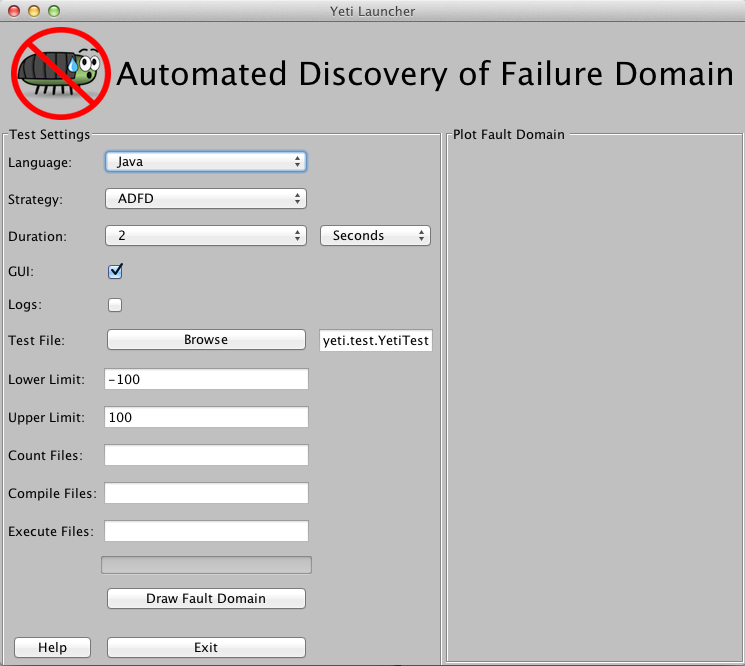
\includegraphics[width=8.2cm,height=4.5cm]{ADFD-front-end.png}
\caption{Front-end of ADFD strategy}
\label{fig:ADFD}
\end{figure}


The process is divided into the following four major parts for simplification. Each part is explained below.

\begin{enumerate}
\item Providing Input From GUI Front-end
\item Automated Fault Finding
\item Automated generation of modules
\item Automated compilation and execution of modules
\item Automated Generation of Graph
\end{enumerate}

\begin{figure}[ht]
\centering
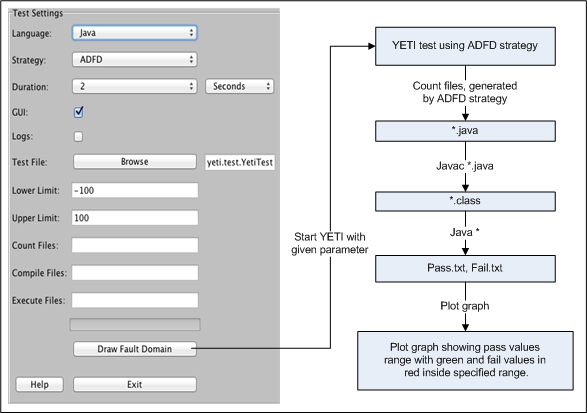
\includegraphics[width=8.2cm,height=6cm]{ADFD-Diagram1.png}
\caption{Working Flow of ADFD strategy}
\label{fig:ADFD}
\end{figure}

\noindent \textbf{Providing Input From GUI Front-end:}\\*
ADFD strategy is provided with an easy to use GUI front-end to get input from the user. It takes YETI specific input including language of the program, strategy, duration, enable or disable YETI GUI, logs and a program to test in the form of java byte code. In addition it also takes minimum and maximum values for restricting ADFD strategy to search for fault domain in the specified range. Default range for minimum and maximum range is Integer.MIN\_INT and Integer.MAX\_INT respectively. 

\noindent \textbf{Automated Fault Finding:}\\*
\indent To find the failure domain for a specific fault first we need to identify that fault in the system. ADFD strategy uses random+ strategy --- random strategy with preference to the boundary values for better performance to find the fault. ADFD strategy is implemented in York Extensible Testing Infrastructure (YETI). The ADFD strategy is implemented in automated testing tool YETI for its simplicity, speed and proven capability of finding potentially hazardous faults in many systems \ref{}. YETI is quick and can call up to one million instructions in one second on Java code. It is also capable of testing VB.Net, C, JML and CoFoJa beside Java. 


\noindent \textbf{Automated generation of modules:}\\*
\indent  After a fault is found in the SUT, ADFD strategy generate complete new Java program to search for fault domain in the given SUT.  These program with .java extension are generated through dynamic compiler API included with Java 6 under javax.tools package. The number of programs generated can be one or many depending on the number of arguments in the test module i.e. for module with one argument one program is generated, for two argument two programs and so on.
To track fault domain we kept one or more argument constant and one argument variable in the generated program.

\noindent \textbf{Automated compilation and execution of modules:}\\*
\indent  The java programs generated in previous step are compiled using javac command to get their binary (.class) files. After that the (java *) command is executed to execute the compiled programs. During execution the constant arguments of the module remain the same but the variable argument receive all the values specified at the start from minimum to maximum. After execution is complete we get two text files of pass and fail. Pass file contain all the values for which the module behave correctly while Fail file contain the values for which the modules failed.\\

\noindent \textbf{Automated Generation of Graph:}\\*
\indent The values from the pass and fail files are plotted on an (x y) graph using a free open source JFreeChart. For one argument program the y component is kept constant. The pass values are represented with green lines while the fault values are represented using red line on the chart.  Resultant graph clearly depicts the domain of the fault. The graph shows red points in case the program fails for only one value, blocks for failing multiple values and strip for failing long range of values.\\


\begin{comment}


%\begin{center}
%\begin{figure*}[htp]
%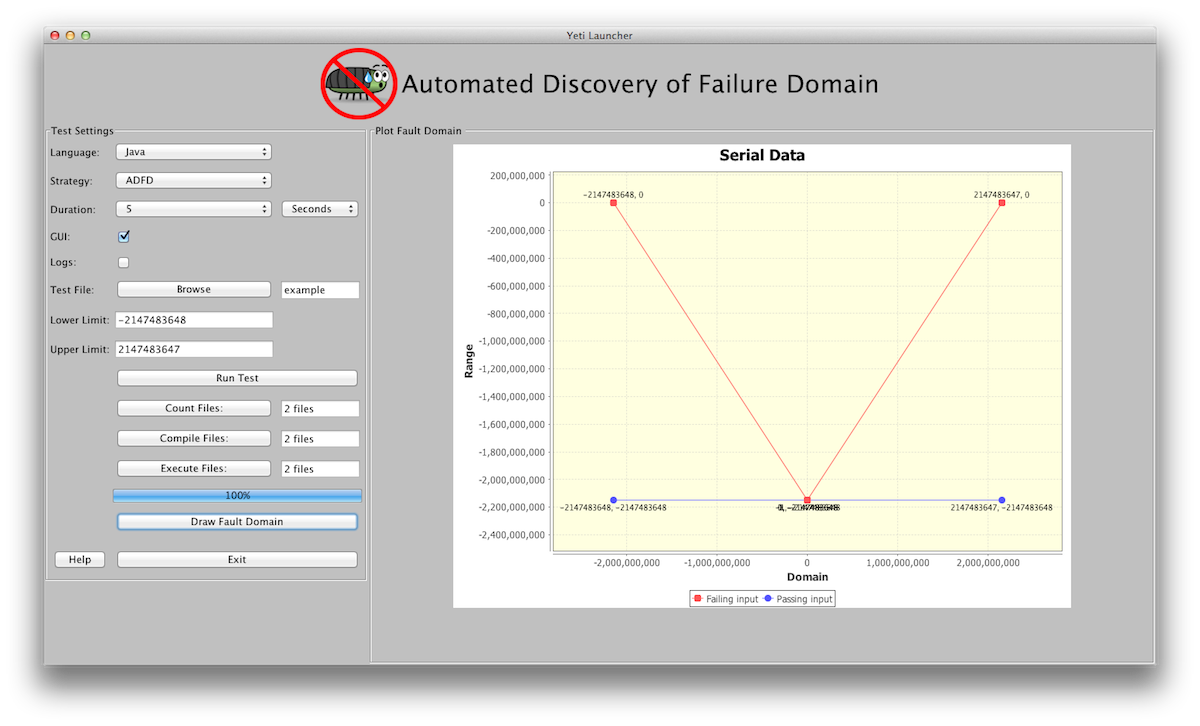
\includegraphics[width=17cm,height=10cm]{adfdFrontEnd.png}
%\caption{GUI of ADFD strategy}
%\label{fig:patterns}
%\end{figure*}
%\end{center}

%\begin{center}
\begin{table}[ht]
%\renewcommand{\arraystretch}{2}
\centering
{\small} 
%\normalsize
\scriptsize
\begin{tabular}{|l|}

\hline 
current\_faults: INTEGER\\
old\_faults: INTEGER\\
...\\
\\
current\_faults := track\_number\_of\_errors\\
old\_faults := 0\\
if ( current\_faults > old\_faults)\\
then \\
old\_faults := current\_faults generate a program dynamically \\
with the following algorithm.\\
 ...\\
 \\
 continue testing \\
\hline


\end{tabular}
\bigskip
\caption{Algorithm}

\label{tb:algorithm}
\end{table}
%\end{center}

%%%%%%%%%%%%%%%%%%%%%%%%%%%%%
%%%%%%%%%%%%%%%%%%%%%%%%%%


%\begin{center}
\begin{table}[ht]
%\renewcommand{\arraystretch}{2}
\centering
{\small} 
%\normalsize
\scriptsize
\begin{tabular}{|l|}

\hline 
Begin Class C*

pass: ArrayList<Integer>\\
fail: ArrayList<Integer>\\
startedByFailing: boolean\\
isCurrentlyFailing: boolean\\
start: Integer\\
stop: Integer\\

start := -100\\
stop := 100\\
startedByFailing := false\\
isCurrentlyFailing :=false\\

BEGIN main method




current\_faults := track\_number\_of\_errors\\
old\_faults := 0\\
if ( current\_faults > old\_faults)\\
then \\
old\_faults := current\_faults Generate a program dynamically \\
with the following algorithm.\\
 ...\\
 \\
 continue testing \\
\hline


\end{tabular}
\bigskip
\caption{Algorithm 2}
\label{tb:algorithm2}
\end{table}
%\end{center}

\end{comment}
%\subsection{Flow Chart of the process}

%The following flow chart clearly identify the workflow of the whole process and the various steps involved in the process.

%\begin{figure}[p]
%\centering
%\includegraphics[width=8cm,height=12cm]{automatedFail.png}
%\caption{Automated discovery of Failure Domain}
%\label{fig:autofail}
%\end{figure}




%We found that it is better for the developer to see the range because the fault can be found once but it can generate errors at multiple locations.like point pattern in the first graph only generate fault at location 0 but if the same zero is assigned to second argument then the whole domain values can fail.\\


%\begin{figure}[htp]
%\centering
%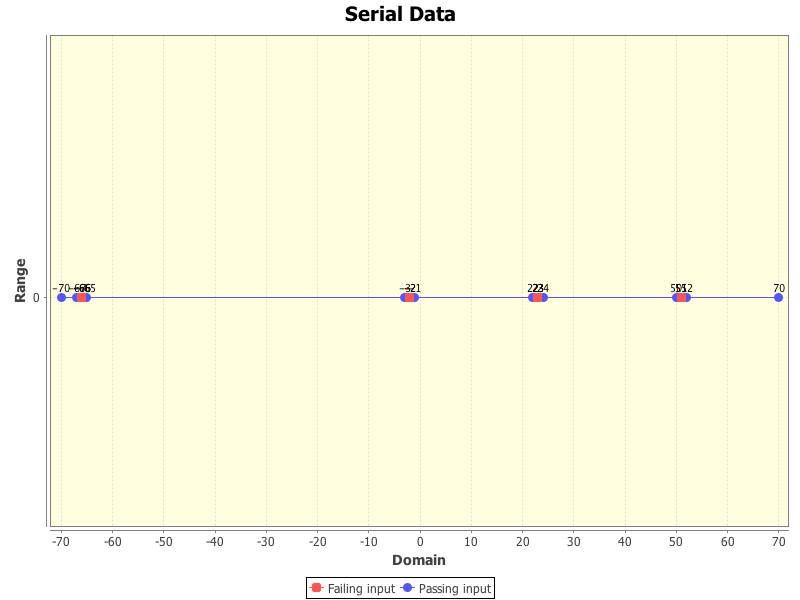
\includegraphics[width=8.5cm,height=6cm]{oneArgumentPointDomain.png}
%\caption{Point pattern failure domain}
%\label{fig:patterns}
%\end{figure}


%Figure \ref{fig:point} shows the example of point pattern. In sub figure \ref{fig1:a} test only fails for 0 out of the whole integer range where as in sub figure \ref{fig1:b} all test fails when static variable is assigned with 0 value.


%\begin{figure}[htp]
%\centering
%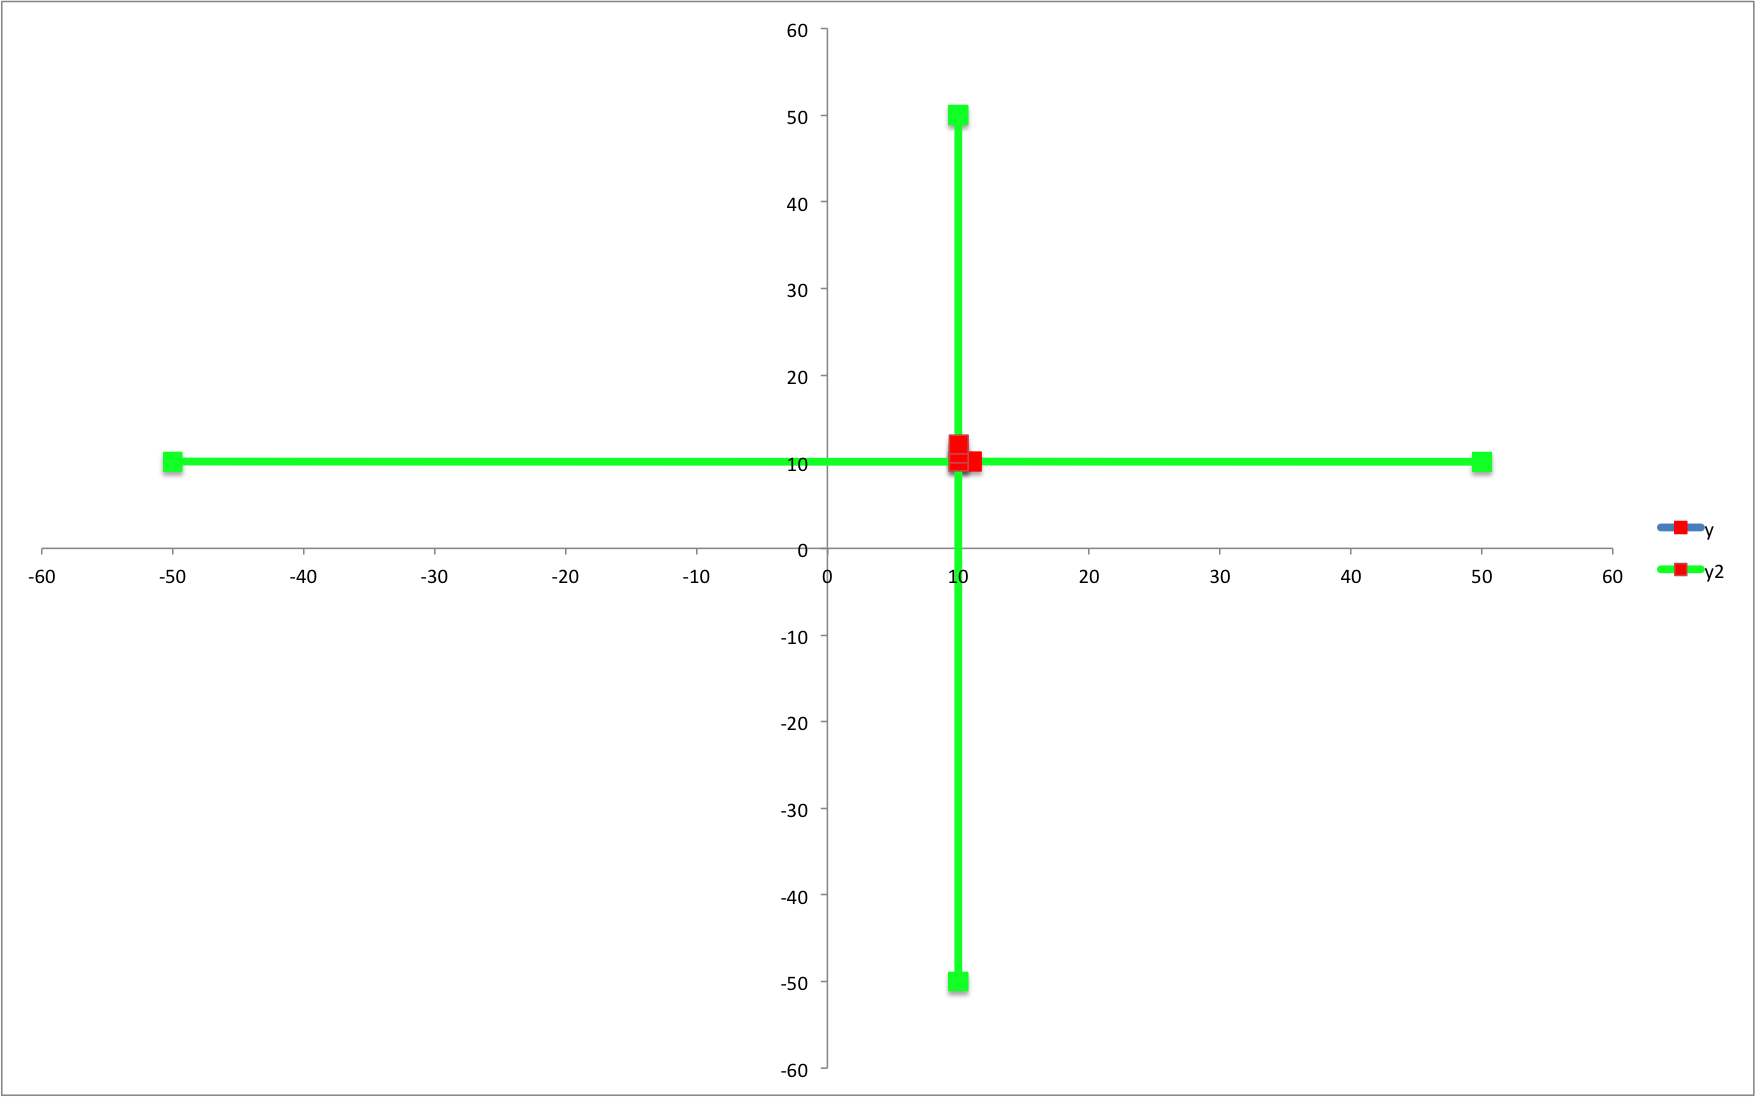
\includegraphics[width=4cm,height=4cm]{block_pattern.png}
%\caption{Block pattern failure domain}
%\label{fig:patterns}
%\end{figure}


%Figure \ref{fig:block} shows the example of block pattern. Both sub figure \ref{fig1:a} and \ref{fig1:b} shows the block pattern of failure. The failure values are given in table \ref{tb:failtable}.

%\begin{figure}[htp]
%\centering
%\begin{center}
%  % Maximum length
 %\subfloat[Test 1 A]{\label{fig1:a}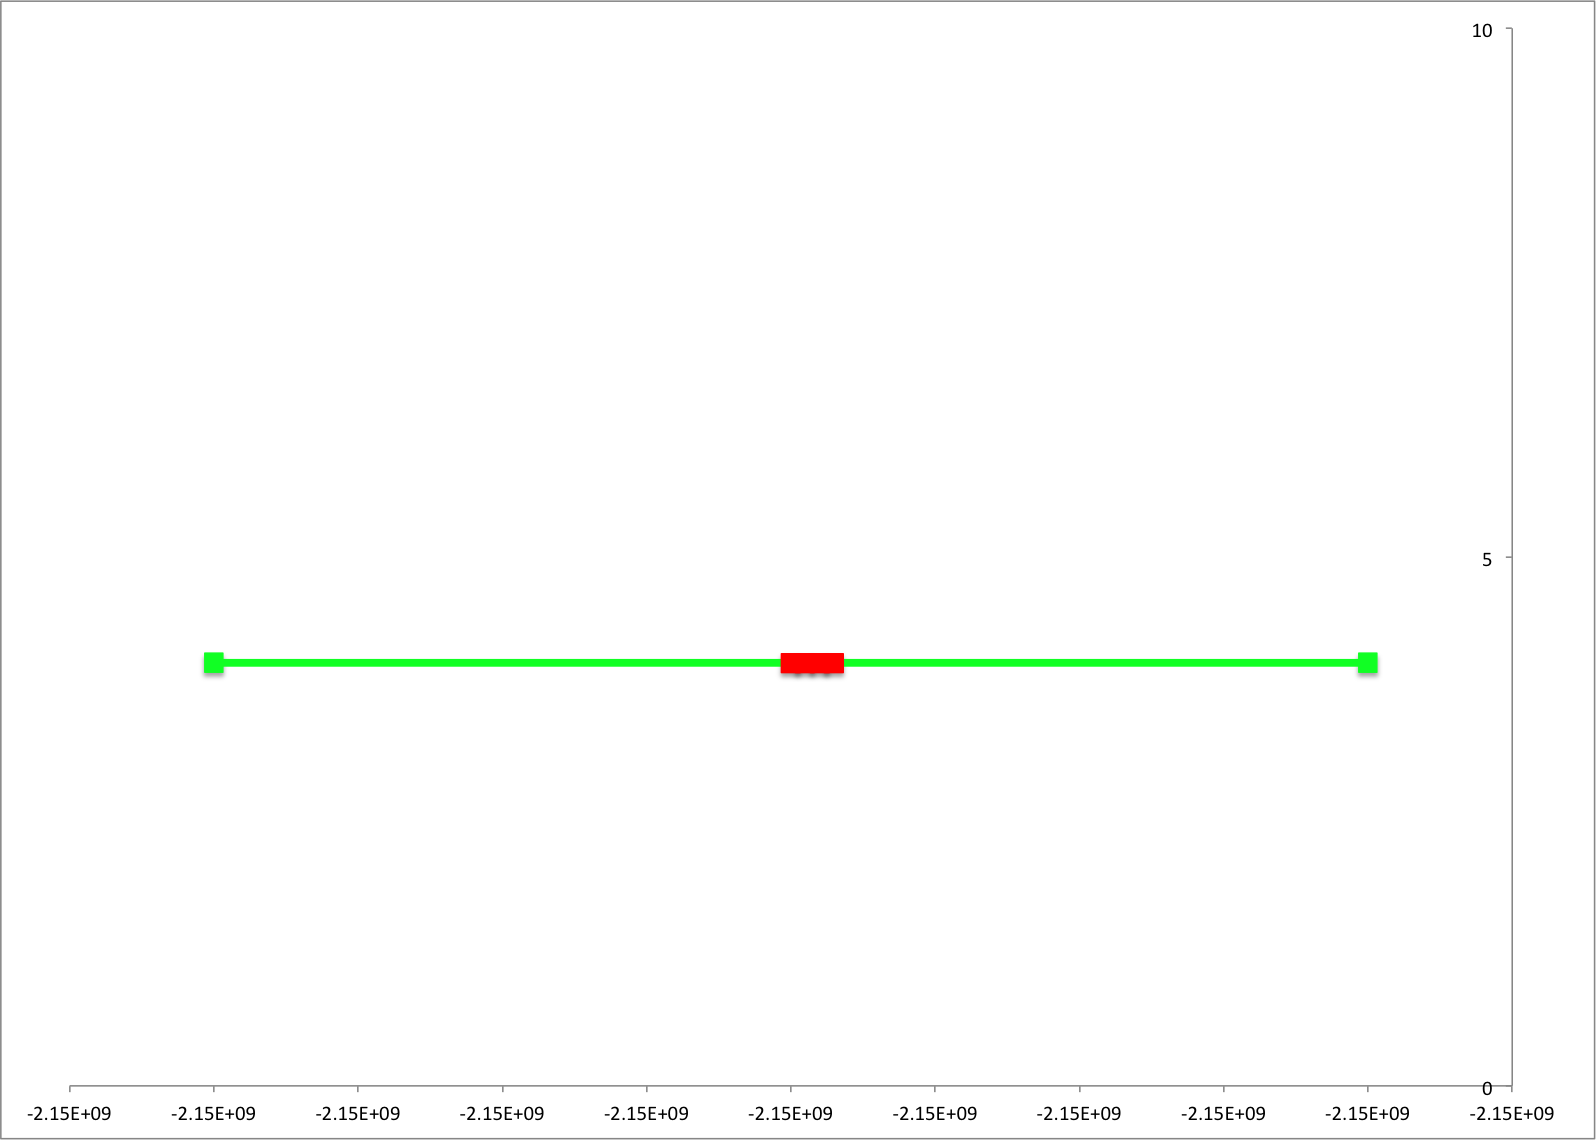
\includegraphics[width=0.49\linewidth]{excel_png/strip_pattern_B.png}}\hfill
 %\subfloat[Test 1 B]{\label{fig1:b}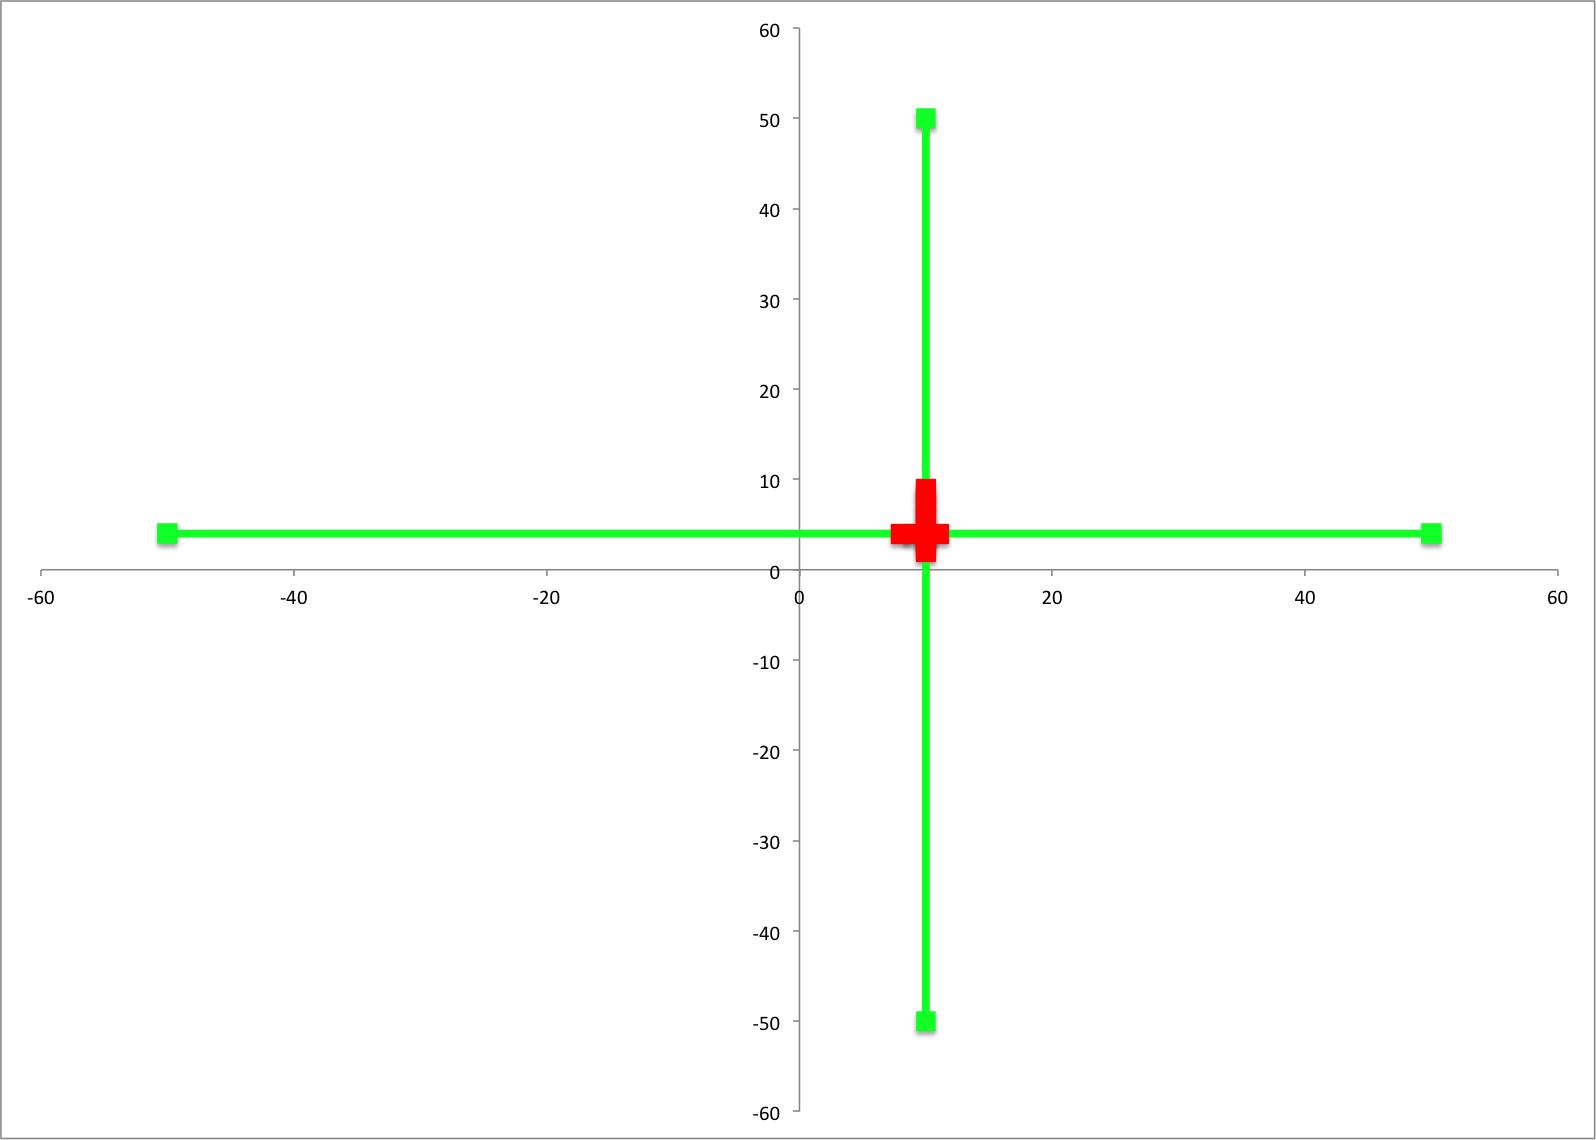
\includegraphics[width=0.49\linewidth]{excel_png/strip_pattern_A.png}}
%  end{center}
%\caption{Strip pattern failure domain}
%%  \label{fig:strip}
%\end{figure}

%Figure shows the example of strip pattern. Here we have two strip failure pattern for test 1 shown in \ref{fig1:a} and \ref{fig1:b} while 1 other for test 2 given in . The failure values are given in table .\\

\section{Implementation}\label{sec:implementation}
 We implemented ADFD strategy in a tool called York Extensible Testing Infrastructure (YETI) \cite{Oriol2010a}. YETI is available in open-source at http://code.google.com/p/yeti-test/. In this section we give a brief overview of YETI, integration of ADFD strategy in YETI and a simple example to illustrate the working of ADFD strategy.

 \subsection{York Extensible Testing Infrastructure}
 It is a testing tool developed in Java that test programs in an automated fashion using random strategies. YETI meta model is language-agnostic which enables it to test programs written in multiple languages that include Java, C\#, JML, .Net and Pharo. YETI consist of three main parts that include the core infrastructure responsible for extendibility through specialisation, the strategies section to adjust multiple strategies and language-specific bindings to provide support for multiple languages \cite{Oriol2010}. 
 
 \subsection{ADFD strategy in YETI}
Strategies package in YETI contain all the strategies including random, random+ and DSSR that can be selected for testing according to the specific needs. The default test strategy for testing is simple random. On top of the hierarchy is an abstract class YetiStrategy which is extended by YetiRandomStrategy and it is further extended to get ADFD strategy as shown in figure \ref{fig:hierarchy}. 
 
\begin{figure}[htp]
\centering
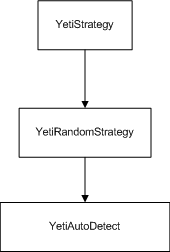
\includegraphics[width=3cm,height=4cm]{Hierarchy1.png}
\caption{Class Hierarchy of automated discovery of failure domains in YETI}
\label{fig:hierarchy}
\end{figure}

\subsection{Example}\label{sec:example}
For a concrete example to show how ADFD strategy in YETI proceeds. We suppose the following class is tested by YETI with ADFD strategy selected for evaluation. Note that for more clear visibility of the output graph generated by ADFD strategy at the end of test session we decrease the values of lower and upper range to -70 and 70 from Integer.Min\_Int and Integer.Max\_Int respectively. 


\begin{lstlisting}
/**
 * Point Fault Domain example for 
 * one argument
 * @author (Mian and Manuel)
 */
public class PointDomainOneArgument{

	public static void pointErrors (int x){
     		if (x == -66)
       			abort();
     
     		if (x == -2)
     			abort();
      				
     		if (x == 51)
     			abort();
     
     		if (x == 23)
     			abort();
	}
}
\end{lstlisting}

%Published programs from literature \cite{Chen2003}\cite{Chan1996}\cite{Chen2004} of point, block and strip failure patterns are tested to explain the working of ADFD . These programs were translated in to java language for this experiment (See appendix 1 for more details). 

As soon as any one of the above four faults are discovered the ADFD strategy generate a dynamic program given in Appendix. This program is automatically compiled to get binary and then executed to find the pass and fail domain inside the specified range as shown in the Figure \ref{fig:ADFD-example}.


\begin{figure}[ht]
\centering
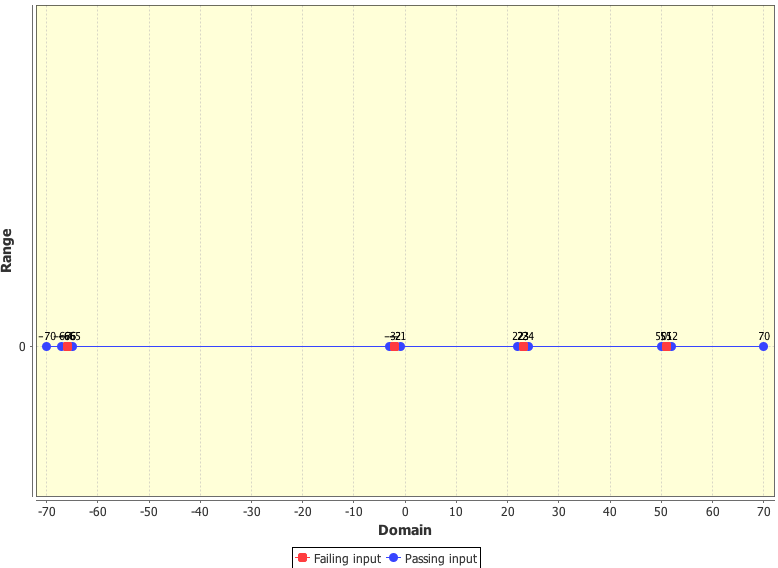
\includegraphics[width=8.2cm,height=5cm]{pointDomainOneArgument.png}
\caption{ADFD strategy plotting pass and fault domain of the given class}
\label{fig:ADFD-example}
\end{figure}



ADFD can be activated by typing the command java -jar ADFD.jar. After the GUI of ADFD is launched we need to specify yeti specific values that include language of the program under test, strategy for the current test session, duration of test session (minutes or milli-second), display YETI GUI or not and display real time logs or not. Next we browse to select the file for testing and the run button starts testing the file with YETI tool. 

In 5 second YETI found one fault out of the above 4 faults. The ADFD strategy in YETI generate a source file (C*.java) at the end of the test session. This file contain the code that searches for fault domains. The count button count the number of files. ADFD create the number of files on the basis of the number of arguments in the method under test. For one argument one method is created and for two argument two methods are created. 

The next button is compile which compile the generated files and generate the byte code (.class files). The execute button execute the byte code and test the method under test for all the values between upper and lower bound. At the end of execution it generates two files (pass.txt and fail.txt). Pass file contain all the values for which the method performed correctly while fail file contain all the values for which the method under test fail.

The draw fault domain button reads the pass and fail files and plot them on the x, y graph where red line with squares show the failing values while the blue line with square shapes show the passing values.

From the figure {} we can see that the use of ADFD not only found all the faults but from the graph we can also know that the program follows a point domain of failure.

%%%%%%%%%%%%%%%%%%%%%%%%%%%%%%%%%%%%%%%%%%%%%%%%%%%%%%%%%%




\section{Experimental Results} \label{sec:experimentalResults}
In this section we present the experimental setup and results of the several experiments performed using ADFD strategy. We selected 10 numerical programs of one and two dimension. These program are error seeded in such a way that they form all the three forms of fault domains that include point, block and strip fault domain. Each selected program contain various combinations of same or different fault domain. Code of the programs is given in Appendix. 

All experiments were performed on a 64-bit Mac OS X Lion Version 10.7.5 running on 2 x 2.66 GHz 6-Core Intel Xeon with 6.00 GB (1333 MHz DDR3) of RAM. YETI runs on top of the Java\texttrademark  SE Runtime Environment [version 1.6.0\_35]. 

For clarification purpose we have taken a separate example program to represent each module. The code of selected programs is given in Appendix. Table \ref{tab:failtable} shows the results of the experiments. We can categorise the results in the following four parts.

%\begin{center}
\begin{table*}[t]
%\renewcommand{\arraystretch}{2}
\centering
\small 
%normalsize

\begin{tabular}{|c|c|c|l|l|l|}

\hline 


S. No		& Fault Domain	 				& Module Dimension 		& Specific Fault	 		& Pass Domain 					& Fail Domain 			\\ \hline 

\multirow{4}{*}{1} 	&	\multirow{4}{*}{Point}		& 	\multirow{2}{*}{One}			&	\multirow{2}{*}{PFDOneA(i)}	&	-100 - -67, -65 - -3, -1 - 50,  			& -66, -2, 23, 51			 	\\  
				&									&							&							&	2 - 22, 24 - 50, 52 - 100				&							\\  \cline{3-6}
				&									&	\multirow{2}{*}{Two}			&	PFDTwoA(2, i)				&	(2, 100) - (2, 1),	 (2, -1) - (2, -100)		&  (2, 0)						\\  \cline{4-6}
				&									& 							&	PFDTwoA(i, 0)				&	Nil								& (-100, 0) - (100, 0)				\\  \hline



\multirow{4}{*}{2} 	&	\multirow{4}{*}{Block}		& 	\multirow{2}{*}{One}			&	\multirow{2}{*}{BFDOneA(i)}	&	-100 - -30, -25 - -2, 					& 	-1 - 1, -29 - -24,		 	\\ 
				&									&							&							&	2 - 50, 55 - 100						&	51 - 54,				\\  \cline{3-6}
				&									&	\multirow{2}{*}{Two}			&	BFDTwoA(-2, i)				&	(-2, 100) - (-2, 20), (-2, -1) - (-2, -100)	& 	(-2 , 1) - ( -2, 19), (-2, 0)		\\  \cline{4-6}
				&									& 							&	BFDTwoA(i, 0)				&	Nil								& 	(-100, 0) - (100, 0)		\\  \hline
				
				



\multirow{4}{*}{3} 	&	\multirow{4}{*}{Strip}		& 	\multirow{2}{*}{One}			&	\multirow{2}{*}{SFDOneA(i)}	&	\multirow{2}{*}{-100 - -5, 35 - 100}		& 	\multirow{2}{*}{-4, 34	}\\ 
				&									&							&							&									&				\\  \cline{3-6}
				&									&	\multirow{2}{*}{Two}			&	SFDTwoA(-5, i)				&	(-5, 100) - (-5, 40), (-5, 0) - (-5, -100)		&  (-5, 39) - (-5, 1), (-5, 0)			\\  \cline{4-6}
				&									& 							&	SFDTwoA(i, 0)				&	Nil								&  (-100, 0) - (100, 0)			\\  \hline
				
				
\end{tabular}
\bigskip
\caption{Pass and Fail domain with respect to one and two dimensional program}
\label{tab:failtable}
\end{table*}
%\end{center}



\textbf{Point Fault Domain:}  Two separate programs P1 and P2 ( Appendix ) were tested with ADFD strategy in YETI to get the chart for point fault domain in one and two dimension program. Figure \ref{fig:PFDOne} represent point fault domain in one dimension whereas Figure \ref{fig:PFDTwo} represent point fault domain in two dimension program. ADFD strategy present ranges for pass and fail values for each program in both text (Table \ref{tab:failtable}, Serial No. 1) and graphical form (Figure \ref{fig:PFDOne} and \ref{fig:PFDTwo}). 
\begin{figure}[H]
\centering
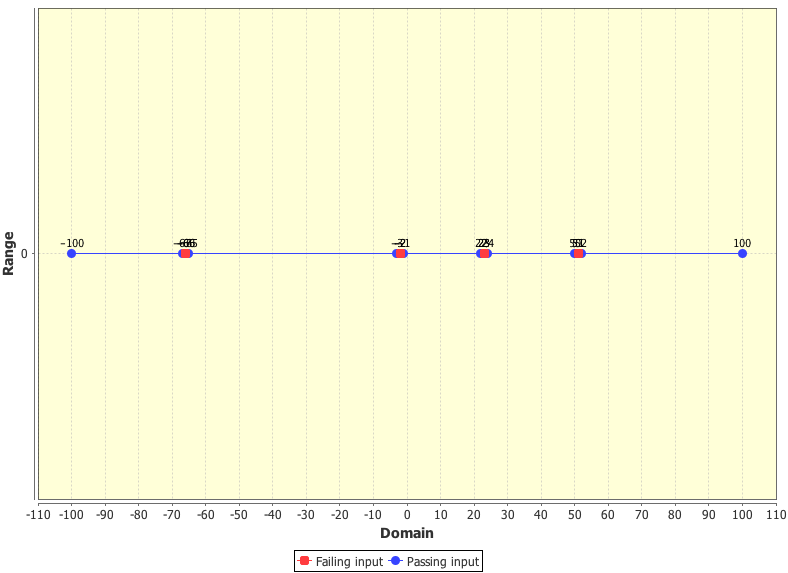
\includegraphics[width=8.2cm,height=5cm]{PFDOne.png}
\caption{Chart generated by ADFD strategy presenting point fault domain in one dimension module}
\label{fig:PFDOne}
\end{figure}

\begin{figure}[H]
\centering
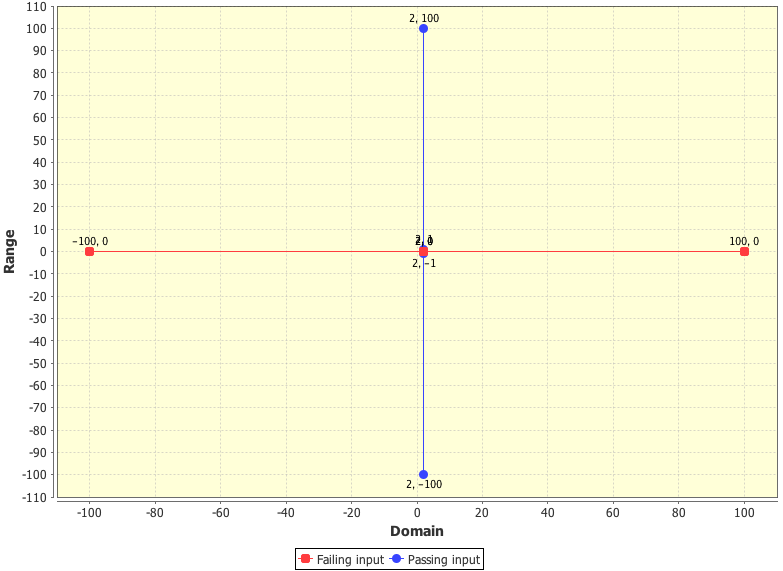
\includegraphics[width=8.2cm,height=5cm]{PFDTwo.png}
\caption{Chart generated by ADFD strategy presenting point fault domain in two dimension module}
\label{fig:PFDTwo}
\end{figure}


\textbf{Block Fault Domain:} Two programs P1 and P2 ( Appendix ) of one and two dimension are tested to get Figure \ref{fig:BFDOne} and \ref{fig:BFDTwo} representing block fault domain. The pass and fail values for each block fault program is given in (Table \ref{tab:failtable}, Serial No. 2).

\begin{figure}[H]
\centering
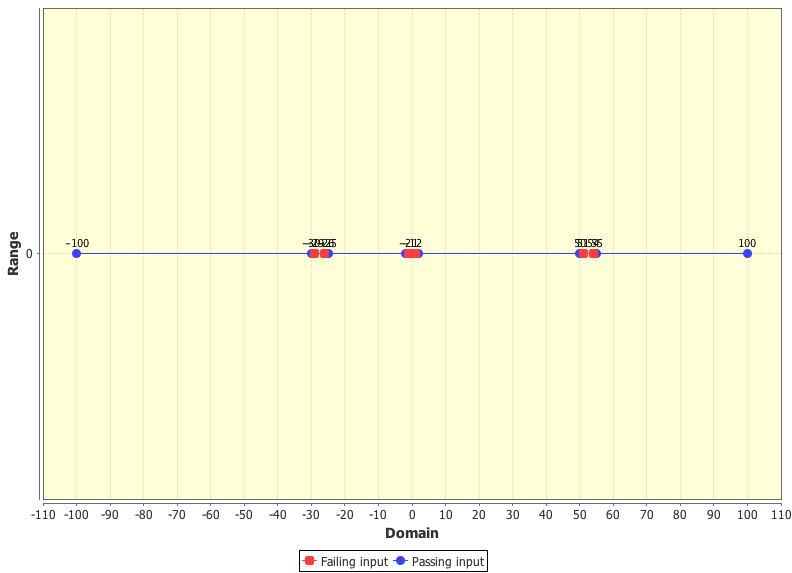
\includegraphics[width=8.2cm,height=5cm]{BFDOne.png}
\caption{Chart generated by ADFD strategy presenting block fault domain in one dimension module}
\label{fig:BFDOne}
\end{figure}


\begin{figure}[H]
\centering
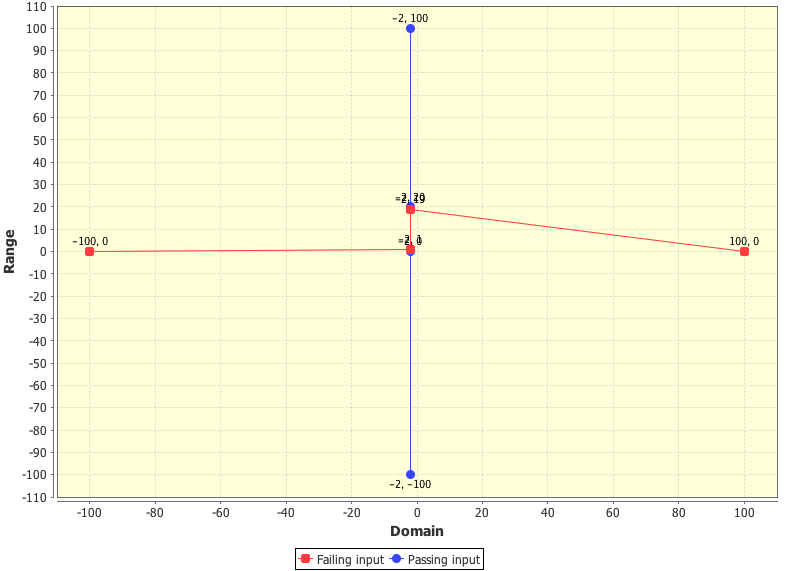
\includegraphics[width=8.2cm,height=5cm]{BFDTwo.png}
\caption{Chart generated by ADFD strategy presenting block fault domain in two dimension module}
\label{fig:BFDTwo}
\end{figure}



\textbf{Strip Fault Domain:} Two programs P1 and P2 ( Appendix ) of one and two dimension are tested to get Figure \ref{fig:SFDOne} and \ref{fig:SFDTwo} representing strip fault domain. The pass and fail values for each strip fault program is given in (Table \ref{tab:failtable}, Serial No. 3).



\begin{figure}[H]
\centering
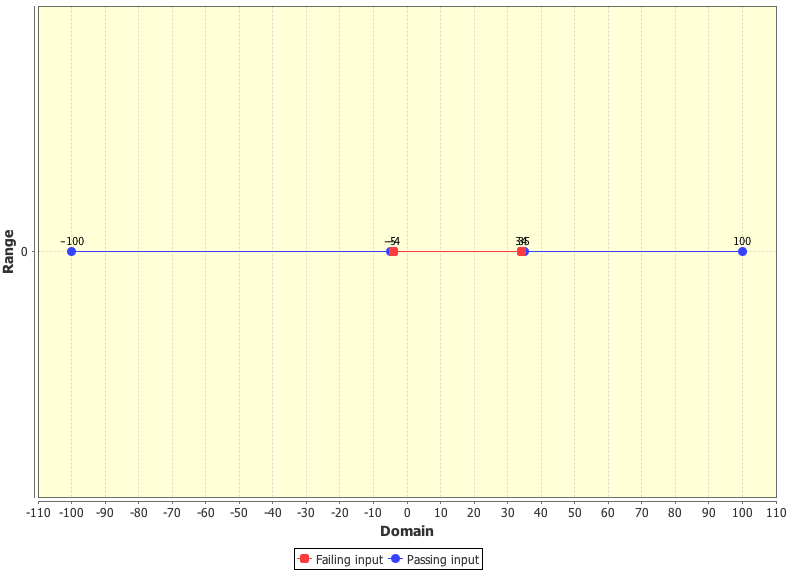
\includegraphics[width=8.2cm,height=5cm]{SFDOne.png}
\caption{Chart generated by ADFD strategy presenting strip fault domain in one dimension module}
\label{fig:SFDOne}
\end{figure}

\begin{figure}[H]
\centering
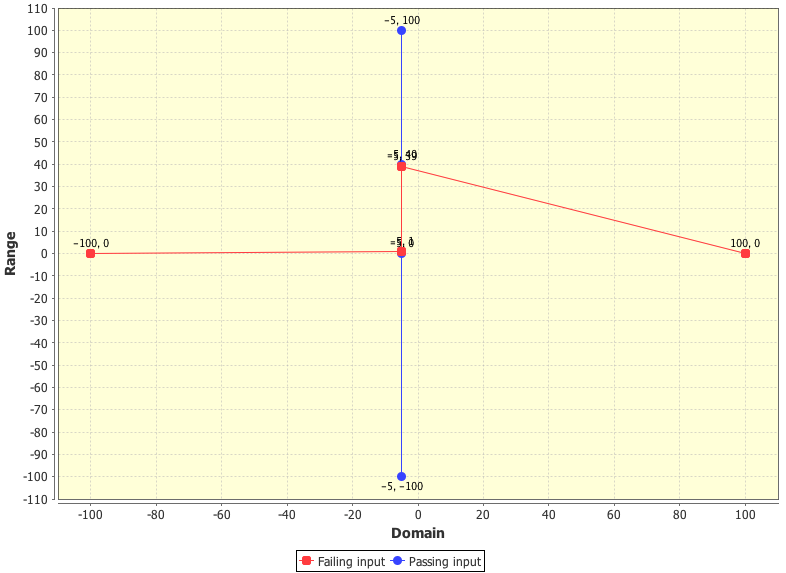
\includegraphics[width=8.2cm,height=5cm]{SFDTwo.png}
\caption{Chart generated by ADFD strategy presenting strip fault domain in two dimension module}
\label{fig:SFDTwo}
\end{figure}


\textbf{ Hybrid Fault Domain in one and ---- Dimension }



\section{Discussion} \label{sec:discussion}

ADFD strategy with a simple graphical user interface is a completely automated process to identify and plot the pass and fault domains on the chart. Since the default settings are all set to optimum the user needs only to specify the module to be tested and click ''plot domain" button to plot domains.

ADFD strategy can effectively identify faults and faults domain in a program. Identification of fault domain is simple for one and two dimension numerical program but the difficulty increases as the program dimension increases beyond two. Similarly no clear boundaries are defined for non numerical data therefore it is not possible to plot domains for non numerical data unless some boundary criteria is defined.

ADFD strategy initiate testing with random+ strategy to find the fault and later switch to brute-force testing to apply all the values between upper and lower bound for finding pass and fault domain.

The main factor dependant on test execution time is the lower and upper bound. If the lower and upper bound is set to maximum or whole input domain then the test duration is maximum. Beside this test duration is also influenced by the identification of the fault and the complexity of module under test.

ADFD strategy can help the debuggers in two ways. First, it reduces the to and from movement of the project between the testers and debuggers as it identity all the faults in one go. Second, it identify locations of all fault domains across the input domain in a user friendly way helping debugger to fix the fault keeping in view its all occurrences.





\section{Related Work} \label{sec:relatedWork}



\section{Conclusion} \label{sec:conclusion}
One conclusion is that ARDT helps in exploring new faults or you can say new failure test cases because if you see figure 3 (a, b, c) it gives 3 range of values for which the program fails. \\

Doing this also saves time in debugging because in ordinary testing the testing stops as soon as the fault is discovered and once the fault is removed by the developers the testing starts again. But here the develop debug the program for all the range instead of single fault value thus saving multiple steps. \\


Debugging can also be made more efficient because the debugger will have the list of all the values for which the program fail therefore he will be in a more better position to rectify the faults and test them against those special values before doing any further testing.\\

We also found that the block and strip pattern are most common in arithmatic programs where as point pattern are more frequently found in general programs. \\

This study will also let us know the reality of failure patterns and its existence across the programs.


%ACKNOWLEDGMENTS are optional
\section{Acknowledgments} \label{sec:acknowledgments}
This section is optional; it is a location for you
to acknowledge grants, funding, editing assistance and
what have you.  In the present case, for example, the
authors would like to thank Gerald Murray of ACM for
his help in codifying this \textit{Author's Guide}
and the \textbf{.cls} and \textbf{.tex} files that it describes.

%
% The following two commands are all you need in the
% initial runs of your .tex file to
% produce the bibliography for the citations in your paper.
\bibliographystyle{abbrv}
\bibliography{sigproc}  % sigproc.bib is the name of the Bibliography in this case
% You must have a proper ".bib" file
%  and remember to run:
% latex bibtex latex latex
% to resolve all references
%
% ACM needs 'a single self-contained file'!
%
%APPENDICES are optional
%\balancecolumns


\onecolumn
\appendix
\bigskip
%\lstset{basicstyle=\tiny}

\begin{lstlisting}
/**
 * Dynamically generated code by ADFD strategy
 * @author (Mian and Manuel)
 */
import java.io.*;
import java.util.*;

public class C0 
{
 public static ArrayList<Integer> pass = new ArrayList<Integer>();
 public static ArrayList<Integer> fail = new ArrayList<Integer>();
 public static boolean startedByFailing = false;
 public static boolean isCurrentlyFailing = false;
 public static int start = -80; 
 public static int stop = 80;

 public static void main(String []argv){
  checkStartAndStopValue(start);
  for (int i=start+1;i<stop;i++){
   try{
PointDomainOneArgument.pointErrors(i);
   if (isCurrentlyFailing) 
  {
fail.add(i-1);
fail.add(0);
pass.add(i);
pass.add(0);
  isCurrentlyFailing=false; 
  } 
 } 
  catch(Throwable t) { 
  if (!isCurrentlyFailing) 
  {
pass.add(i-1);
pass.add(0);
fail.add(i);
fail.add(0);
isCurrentlyFailing = true;
 }  
 } 
 } 
 checkStartAndStopValue(stop); 
  printRangeFail(); 
  printRangePass();  
  }

 public static void printRangeFail() { 
   try { 
   File fw = new File("Fail.txt"); 
   if (fw.exists() == false) { 
 	 fw.createNewFile(); 
   }
	 PrintWriter pw = new PrintWriter(new FileWriter (fw, true));   
	 for (Integer i1 : fail) { 
      pw.append(i1+"\n"); 
   } 
   pw.close(); 
   } 
   catch(Exception e) { 
   System.err.println(" Error : e.getMessage() "); 
   } 
 } 
  public static void printRangePass() { 
   try { 
   File fw1 = new File("Pass.txt"); 
   if (fw1.exists() == false) { 
 	 fw1.createNewFile(); 
   }
	 PrintWriter pw1 = new PrintWriter(new FileWriter (fw1, true));   for (Integer i2 : pass) { 
      pw1.append(i2+"\n");
   } 
   pw1.close(); 
   } 
   catch(Exception e) { 
   System.err.println(" Error : e.getMessage() "); 
   } 
 } 
   public static void checkStartAndStopValue(int i) { 
   try { 
   PointDomainOneArgument.pointErrors(i);
 pass.add(i); 
pass.add(0);
  } 
  catch (Throwable t) { 
  startedByFailing = true; 
  isCurrentlyFailing = true; 
  fail.add(i); 
 fail.add(0);
 } 
 } 
}
\end{lstlisting}

% That's all folks!
\end{document}
